
\begin{enumerate}[label=\thechapter.\arabic*,ref=\thechapter.\theenumi]
\numberwithin{equation}{enumi}
\numberwithin{figure}{enumi}
\numberwithin{table}{enumi}
\item
\label{12/6/6/22}
\iffalse
\documentclass[journal,10pt,twocolumn]{article}
\usepackage{graphicx, float}
\usepackage[margin=0.5in]{geometry}
\usepackage{amsmath, bm}
\usepackage{array}
\usepackage{booktabs}
\usepackage[utf8]{inputenc}
\usepackage{amsfonts}
\usepackage{amssymb}
\usepackage{graphicx}
\usepackage{multicol}
\usepackage{tabularx}
\usepackage{hyperref}
\usepackage{mathtools}
\DeclareUnicodeCharacter{2212}{-}
\providecommand{\norm}[1]{\left\lVert#1\right\rVert}
\providecommand{\abs}[1]{\left\vert#1\right\vert}
\let\vec\mathbf
\newcommand{\myvec}[1]{\ensuremath{\begin{pmatrix}#1\end{pmatrix}}}
\newcommand{\mydet}[1]{\ensuremath{\begin{vmatrix}#1\end{vmatrix}}}
\providecommand{\brak}[1]{\ensuremath{\left(#1\right)}}
\providecommand{\lbrak}[1]{\ensuremath{\left(#1\right.}}
\providecommand{\rbrak}[1]{\ensuremath{\left.#1\right)}}
\providecommand{\sbrak}[1]{\ensuremath{{}\left[#1\right]}}
%\providecommand{\norm}[1]{\left\lVert#1\right\rVert}
%\providecommand{\sbrak}[1]{\ensuremath{{}\left[#1\right]}}
%\providecommand{\lsbrak}[1]{\ensuremath{{}\left[#1\right.}}
%\providecommand{\rsbrak}[1]{\ensuremath{{}\left.#1\right]}}
%\providecommand{\brak}[1]{\ensuremath{\left(#1\right)}}
%\providecommand{\lbrak}[1]{\ensuremath{\left(#1\right.}}
%\providecommand{\rbrak}[1]{\ensuremath{\left.#1\right)}}
%\providecommand{\cbrak}[1]{\ensuremath{\left\{#1\right\}}}
%\providecommand{\lcbrak}[1]{\ensuremath{\left\{#1\right.}}
%\providecommand{\rcbrak}[1]{\ensuremath{\left.#1\right\}}}
%\newcommand{\myvec}[1]{\ensuremath{\begin{pmatrix}#1\end{pmatrix}}}
%\let\vec\mathbf

\title{\textbf{Optimization Assignment}}
\author{Jyothsna Paluchuri \hspace{9cm} FWC22059}


\begin{document}

\maketitle
\paragraph{\textit{Problem Statement} -
\fi
Find the normal to the curve $2y+x^2=3$ passing through (2,2). 
\\
\solution 
\iffalse
:\\
(a)x+y=0  \hspace{2cm} (b)x-y=0\\ 
(c)x+y+1=0 \hspace{2cm}  (d)x-y=1\\}
\section*{\large Solution}

\begin{figure}[H]
\centering
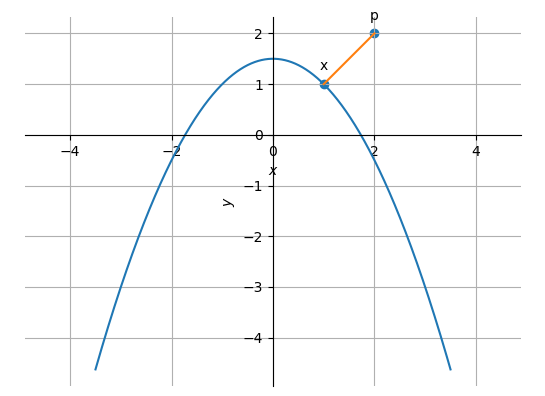
\includegraphics[width=1\columnwidth]{opt.png}
\caption{Normal to the curve $x^2+2y=3$}
\end{figure}

The given equation of parabola $x^2+2y=3$ can be written in the general quadratic form as
\begin{align}
    \vec{x}^{\top}\vec{V}\vec{x}+2\vec{u}^{\top}\vec{x}+f=0
    \end{align}
where
\fi
The parameters of the given conic are
\begin{align}
	\label{eq:12/6/6/22V_matrix}
	\vec{V} = \myvec{1 & 0\\0 & 0},
	\vec{u} = \myvec{0\\1},
	f =-3
\end{align}
If $\vec{x}$ be the point of contact on the conic, the optimization problem can be formulated as 
\begin{align}
	\label{eq:12/6/6/22/quad}
	\vec{q} = \min_{\vec{x}}\norm{\vec{x}-\vec{p}}^2
	\\
	s.t. \quad 
    \vec{x}^{\top}\vec{V}\vec{x}+2\vec{u}^{\top}\vec{x}+f=0
    \label{eq:12/6/6/22conic_quad_form}
\end{align}
%
where 
\begin{align}
	\vec{p} = \myvec{2 \\ 2}
\end{align}
Since 
\begin{align}
	\norm{\vec{x}-\vec{p}}^2 &= 
	\norm{\vec{x}}^2 - 2\vec{p}^{\top}\vec{x} + \norm{\vec{p}}^2
	\\
	&= 
\vec{y}^{\top}\vec{C}\vec{y}
\end{align}
\iffalse
\begin{center}
 Any conic of the form  $\vec{x^{\top}}\vec{V}\vec{x} + 2\vec{u^{\top}}\vec{x} + f = 0$ \end{center}
\begin{center} can be written as $\vec{x^{\top}}\vec{A}\vec{x} = 0$\end{center} 
\begin{center}
where $\vec{A} = \myvec{\vec{V}&\vec{u}\\\vec{u^{\top}}&f}$, $\vec{x} =\myvec{x\\y\\1}$
\end{center}
\begin{center}
The distance from point $\vec{p} = \myvec{2\\2}$ to the point 'x' on parabola is $\|\vec{x}-\vec{p}\|^2$
\end{center}

\begin{gather*}
	\implies 
\end{gather*}

\begin{center}
	\fi
	where
\begin{align}
	\vec{C} = \myvec{\vec{I}&-\vec{p}\\ -\vec{p}^{\top}& \norm{\vec{p}}^2}\, \vec{y} = \myvec{\vec{x}\\1}
\end{align}
and 
    \eqref{eq:12/6/6/22conic_quad_form} can be expressed as 
\begin{align}
    \vec{y}^{\top}\vec{A}\vec{y}=0,
\end{align}
where
\begin{align}
\vec{A} = \myvec{\vec{V}&\vec{u}\\\vec{u}^{\top}&f},
\end{align}
\iffalse

\begin{center}
The shortest distance is given by, min $\vec{x^{\top}}\vec{C}\vec{x}$
\end{center}
\begin{center}
such that,  $\vec{x^{\top}}\vec{A}\vec{x} = 0$
	\\ \raggedright 
\fi
	Using SDR (Semi Definite Relaxation), 
	\eqref{eq:12/6/6/22/quad}
	can be expressed as
\iffalse
	it can be rewritten as 
	\\ \centering 
\end{center}
\begin{center}
Suc that, $ 
	\fi
\begin{align}
	\min_{\vec{X}} tr\brak{\vec{C}\vec{X}}
	\\
s.t. \quad	tr\brak{\vec{A}\vec{X}} =0,
\\
 \vec{X}\succeq \vec{0}
\end{align}
\iffalse
\end{center}
\begin{center}
Here , $\vec{X}$ is a  $3\times3$ matrix of variables where
	\\ \centering $ \vec{X} = \vec{x}\vec{x^{\top}}$
\end{center}

Thus after solving we get the point on the given parabola as $\vec{x} = \myvec{1\\1}$ with the shortest distance from  $\vec{p}$
\begin{center}
	\fi
	yielding
\begin{align}
\vec{x} = \myvec{1\\1}.
\end{align}
Thus, the 
% and $\vec{p} = \myvec{2\\2}$ satisfies 
equation of the normal is
\begin{align}
	\myvec{1 &-1}\vec{x}=0
\end{align}
\iffalse
\end{center} 

\section*{\large Construction}
{
\setlength\extrarowheight{5pt}
\begin{tabular}{|c|c|c|}
	\hline
	\textbf{Symbol}&\textbf{Value}&\textbf{Description}\\[5pt]
	\hline
	$\vec{p}$&$\myvec{2 \\ 2}$&Given point through which Normal is passing\\[5pt]
	\hline
	$\vec{x}$&$\myvec{1 \\ 1}$&Foot of Normal\\[5pt]
	\hline
\end{tabular}
}

\end{document}
\fi

\item
\label{12/6/6/23}
\iffalse
\documentclass[journal,10pt,twocolumn]{article}
\usepackage{graphicx, float}
\usepackage[margin=0.5in]{geometry}
\usepackage{amsmath, bm}
\usepackage{array}
\usepackage{booktabs}
\usepackage[utf8]{inputenc}
\usepackage{amsfonts}
\usepackage{amssymb}
\usepackage{graphicx}
\usepackage{multicol}
\usepackage{tabularx}
\usepackage{hyperref}
\usepackage{mathtools}
\DeclareUnicodeCharacter{2212}{-}
\providecommand{\norm}[1]{\left\lVert#1\right\rVert}
\providecommand{\abs}[1]{\left\vert#1\right\vert}
\let\vec\mathbf
\newcommand{\myvec}[1]{\ensuremath{\begin{pmatrix}#1\end{pmatrix}}}
\newcommand{\mydet}[1]{\ensuremath{\begin{vmatrix}#1\end{vmatrix}}}
\providecommand{\brak}[1]{\ensuremath{\left(#1\right)}}
\providecommand{\lbrak}[1]{\ensuremath{\left(#1\right.}}
\providecommand{\rbrak}[1]{\ensuremath{\left.#1\right)}}
\providecommand{\sbrak}[1]{\ensuremath{{}\left[#1\right]}}
%\providecommand{\norm}[1]{\left\lVert#1\right\rVert}
%\providecommand{\sbrak}[1]{\ensuremath{{}\left[#1\right]}}
%\providecommand{\lsbrak}[1]{\ensuremath{{}\left[#1\right.}}
%\providecommand{\rsbrak}[1]{\ensuremath{{}\left.#1\right]}}
%\providecommand{\brak}[1]{\ensuremath{\left(#1\right)}}
%\providecommand{\lbrak}[1]{\ensuremath{\left(#1\right.}}
%\providecommand{\rbrak}[1]{\ensuremath{\left.#1\right)}}
%\providecommand{\cbrak}[1]{\ensuremath{\left\{#1\right\}}}
%\providecommand{\lcbrak}[1]{\ensuremath{\left\{#1\right.}}
%\providecommand{\rcbrak}[1]{\ensuremath{\left.#1\right\}}}
%\newcommand{\myvec}[1]{\ensuremath{\begin{pmatrix}#1\end{pmatrix}}}
%\let\vec\mathbf

\title{\textbf{Optimization Assignment}}
\author{Sireesha Abbavaram \hspace{9cm} FWC22060}


\begin{document}

\maketitle
\paragraph{\textit{Problem Statement} - 
\fi
Find the 
normal to the curve $x^2=4y$ passing through (1,2).
\iffalse
(a)x+y=3  \hspace{2cm} (b)x-y=3\\ 
(c)x+y=1 \hspace{2cm}  (d)x-y=1\\}

\section*{\large Solution}

\begin{figure}[H]
\centering
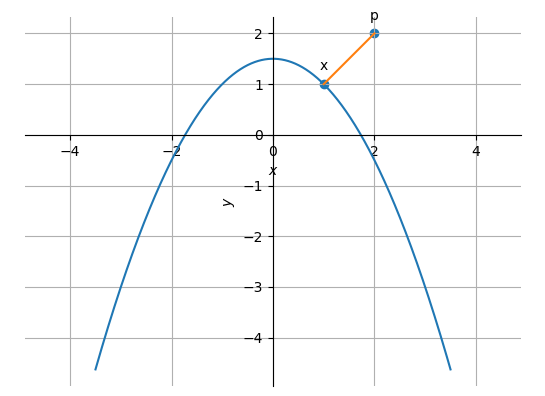
\includegraphics[width=1\columnwidth]{opt.png}
\caption{Normal to the curve $x^2=4y$}
\end{figure}

The given equation of parabola $x^2 = 4y$ can be written in the general quadratic form as
\begin{align}
    \label{eq:conic_quad_form}
    \vec{x}^{\top}\vec{V}\vec{x}+2\vec{u}^{\top}\vec{x}+f=0
    \end{align}
where
\begin{align}
	\label{eq:V_matrix}
	\vec{V} &= \myvec{1 & 0\\0 & 0},
	\\
	\label{eq:u_vector}
	\vec{u} &= \myvec{0\\-2},
	\\
	\label{eq:f_value}
	f &=0
	% ||
\end{align}
\fi
The parameters of the given conic are
\begin{align}
	\label{eq:12/6/6/23V_matrix}
	\vec{V} = \myvec{1 & 0\\0 & 0},
	\vec{u} = \myvec{0\\-2},
	f =0
\end{align}
If $\vec{x}$ be the point of contact on the conic, the optimization problem can be formulated as 
\begin{align}
	\label{eq:12/6/6/23/quad}
	\vec{q} = \min_{\vec{x}}\norm{\vec{x}-\vec{p}}^2
	\\
	s.t. \quad 
    \vec{x}^{\top}\vec{V}\vec{x}+2\vec{u}^{\top}\vec{x}+f=0
    \label{eq:12/6/6/23conic_quad_form}
\end{align}
%
where 
\begin{align}
	\vec{p} = \myvec{1 \\ 2}
\end{align}
Since 
\begin{align}
	\norm{\vec{x}-\vec{p}}^2 &= 
	\norm{\vec{x}}^2 - 2\vec{p}^{\top}\vec{x} + \norm{\vec{p}}^2
	\\
	&= 
\vec{y}^{\top}\vec{C}\vec{y}
\end{align}
	where
\begin{align}
	\vec{C} = \myvec{\vec{I}&-\vec{p}\\ -\vec{p}^{\top}& \norm{\vec{p}}^2}\, \vec{y} = \myvec{\vec{x}\\1}
\end{align}
and 
    \eqref{eq:12/6/6/23conic_quad_form} can be expressed as 
\begin{align}
    \vec{y}^{\top}\vec{A}\vec{y}=0,
\end{align}
where
\begin{align}
\vec{A} = \myvec{\vec{V}&\vec{u}\\\vec{u}^{\top}&f},
\end{align}
	Using SDR (Semi Definite Relaxation), 
	\eqref{eq:12/6/6/23/quad}
	can be expressed as
\begin{align}
	\min_{\vec{X}} tr\brak{\vec{C}\vec{X}}
	\\
s.t. \quad	tr\brak{\vec{A}\vec{X}} =0,
\\
 \vec{X}\succeq \vec{0}
\end{align}
	yielding
\begin{align}
\vec{x} = \myvec{2\\1}.
\end{align}
Thus, the 
% and $\vec{p} = \myvec{2\\2}$ satisfies 
equation of the normal is
\begin{align}
	\myvec{1 &1}\vec{x}=3
\end{align}
\iffalse
\begin{center}
 Any conic of the form  $\vec{x^{\top}}\vec{V}\vec{x} + 2\vec{u^{\top}}\vec{x} + f = 0$ \end{center}
\begin{center} can be written as $\vec{x^{\top}}\vec{A}\vec{x} = 0$\end{center} 
\begin{center}
where $\vec{A} = \myvec{\vec{V}&\vec{u}\\\vec{u^{\top}}&f}$, $\vec{x} =\myvec{x\\y\\1}$
\end{center}
\begin{center}
The distance from point $\vec{p} = \myvec{1\\2}$ to the point 'x' on parabola is $\|\vec{x}-\vec{p}\|^2$
\end{center}

\begin{gather*}
	\implies \vec{x^{\top}}\vec{x} - 2\vec{p^{\top}}\vec{x} + \|\vec{p}\|^2
\end{gather*}

\begin{center}
The above equation can be written as $\vec{x^{\top}}\vec{C}\vec{x}$
\end{center}
\begin{center}
where $\vec{C} = \myvec{\vec{I}&-\vec{p}\\ -\vec{p^{\top}}& \|\vec{p}\|^2}$, $\vec{x} = \myvec{x\\y\\1}$
\end{center}
\begin{center}
The shortest distance is given by, min $\vec{x^{\top}}\vec{C}\vec{x}$
\end{center}
\begin{center}
such that,  $\vec{x^{\top}}\vec{A}\vec{x} = 0$
	\\ \raggedright Using SDR(Semi Definite Relaxation), it can be rewritten as 
	\\ \centering min $Tr\myvec{\vec{C}\vec{X}}$
\end{center}
\begin{center}
Suc that, $ Tr\myvec{\vec{A}\vec{X}} =0,$
 $\vec{X}\ge0$
\end{center}
\begin{center}
Here , $\vec{X}$ is a  $3\times3$ matrix of variables where
	\\ \centering $ \vec{X} = \vec{x}\vec{x^{\top}}$
\end{center}



Thus after solving we get the point on the given parabola as $\vec{x} = \myvec{2\\1}$ with the shortest distance from  $\vec{p}$
\begin{center}
    Thus the points $\vec{x} = \myvec{2\\1}$ and $\vec{p} = \myvec{1\\2}$ satisfies the equation of the normal i.e. $x+y=3$
\end{center} 

\section*{\large Construction}
{
\setlength\extrarowheight{5pt}
\begin{tabular}{|c|c|c|}
	\hline
	\textbf{Symbol}&\textbf{Value}&\textbf{Description}\\[5pt]
	\hline
	$\vec{p}$&$\myvec{1 \\ 2}$&Given point through which Normal is passing\\[5pt]
	\hline
	$\vec{x}$&$\myvec{2 \\ 1}$&Foot of Normal\\[5pt]
	\hline
\end{tabular}
}

\end{document}
\fi

 \item Find the point on the curve 
    \begin{align}
        x^2 = 2y
        \label{eq:12/6/5/27/conv/sdp/curve}
    \end{align}
    which is nearest to the point $\vec{P} = \myvec{2\\1}$.
			\\
\solution 
\label{12/6/5/27/conv/sdp}

 We
    apply the semidefinite relaxation to get the following problem.
    \begin{align}
        \min_{\vec{X}}&\textrm{ tr}\brak{\vec{CX}} \label{eq:12/6/5/27/conv/sdp/sdp-cost} \\
        \textrm{s.t. }&\textrm{ tr}\brak{\vec{AX}} \le 0 \label{eq:12/6/5/27/conv/sdp/sdp-constr} \\
                      &\vec{X} \succeq 0
    \end{align}
    where
    \begin{align}
        \vec{C} &= \myvec{\vec{I}&-\vec{P}\\-\vec{P}^\top&\norm{\vec{P}}^2} \label{eq:12/6/5/27/conv/sdp/C-def} \\
        \vec{A} &= \myvec{\vec{V}&\vec{u}\\\vec{u}^\top&f} \label{eq:12/6/5/27/conv/sdp/A-def}
    \end{align}

    The problem is solved using \textit{cvxpy}. 



\end{enumerate}
